\chapter[2022 June]{June 2022}

\section[2022/06/06]{Monday, 06 June 2022}

\subsection{Further OpenGL Prototyping}

This session focuses on improvements made to the initial OpenGL cube rendering prototype. \\

Further experimentation was performed with the OpenGL library in order to rotate, translate and adjust the virtual object or cube in a desired manner. The \textbf{glTranslatef(x,y,z)} and \textbf{glRotatef(angle,x,y,z)} commands were used to affect the cube in various ways. The perspective system of OpenGL only allows the "camera" or user's perspective to be shifted - not individual objects within the scene. Thus thinking about how to construct the virtual object control system relies upon figuring out how to move the perspective of the camera or point of view as the user provides gesture input. This is further complicated by the fact that the background imagery of the user or scene is merely projected onto an orthographic quad rendered at the back of the OpenGL scene. Thus the idea of a far and near clipping plane must be kept in mind when moving objects between different x,y and z co-ordinates. Getting this background quad rendered and not also moving when the perspective and translation changes are made took many hours of troubleshooting. \\

The completed prototype visible in \FigRef{fig:OpenGL Mediapipe Cube} allows a user to move their hand and the system tracks the location of their pinky finger and attempts to adjust the perspective based on the position of the pinky finger within the camera's frame of view. Further experimentation is needed to adjust the cube at different speeds and produce more realistic output. \\

\begin{figure}[h]
    \centering
    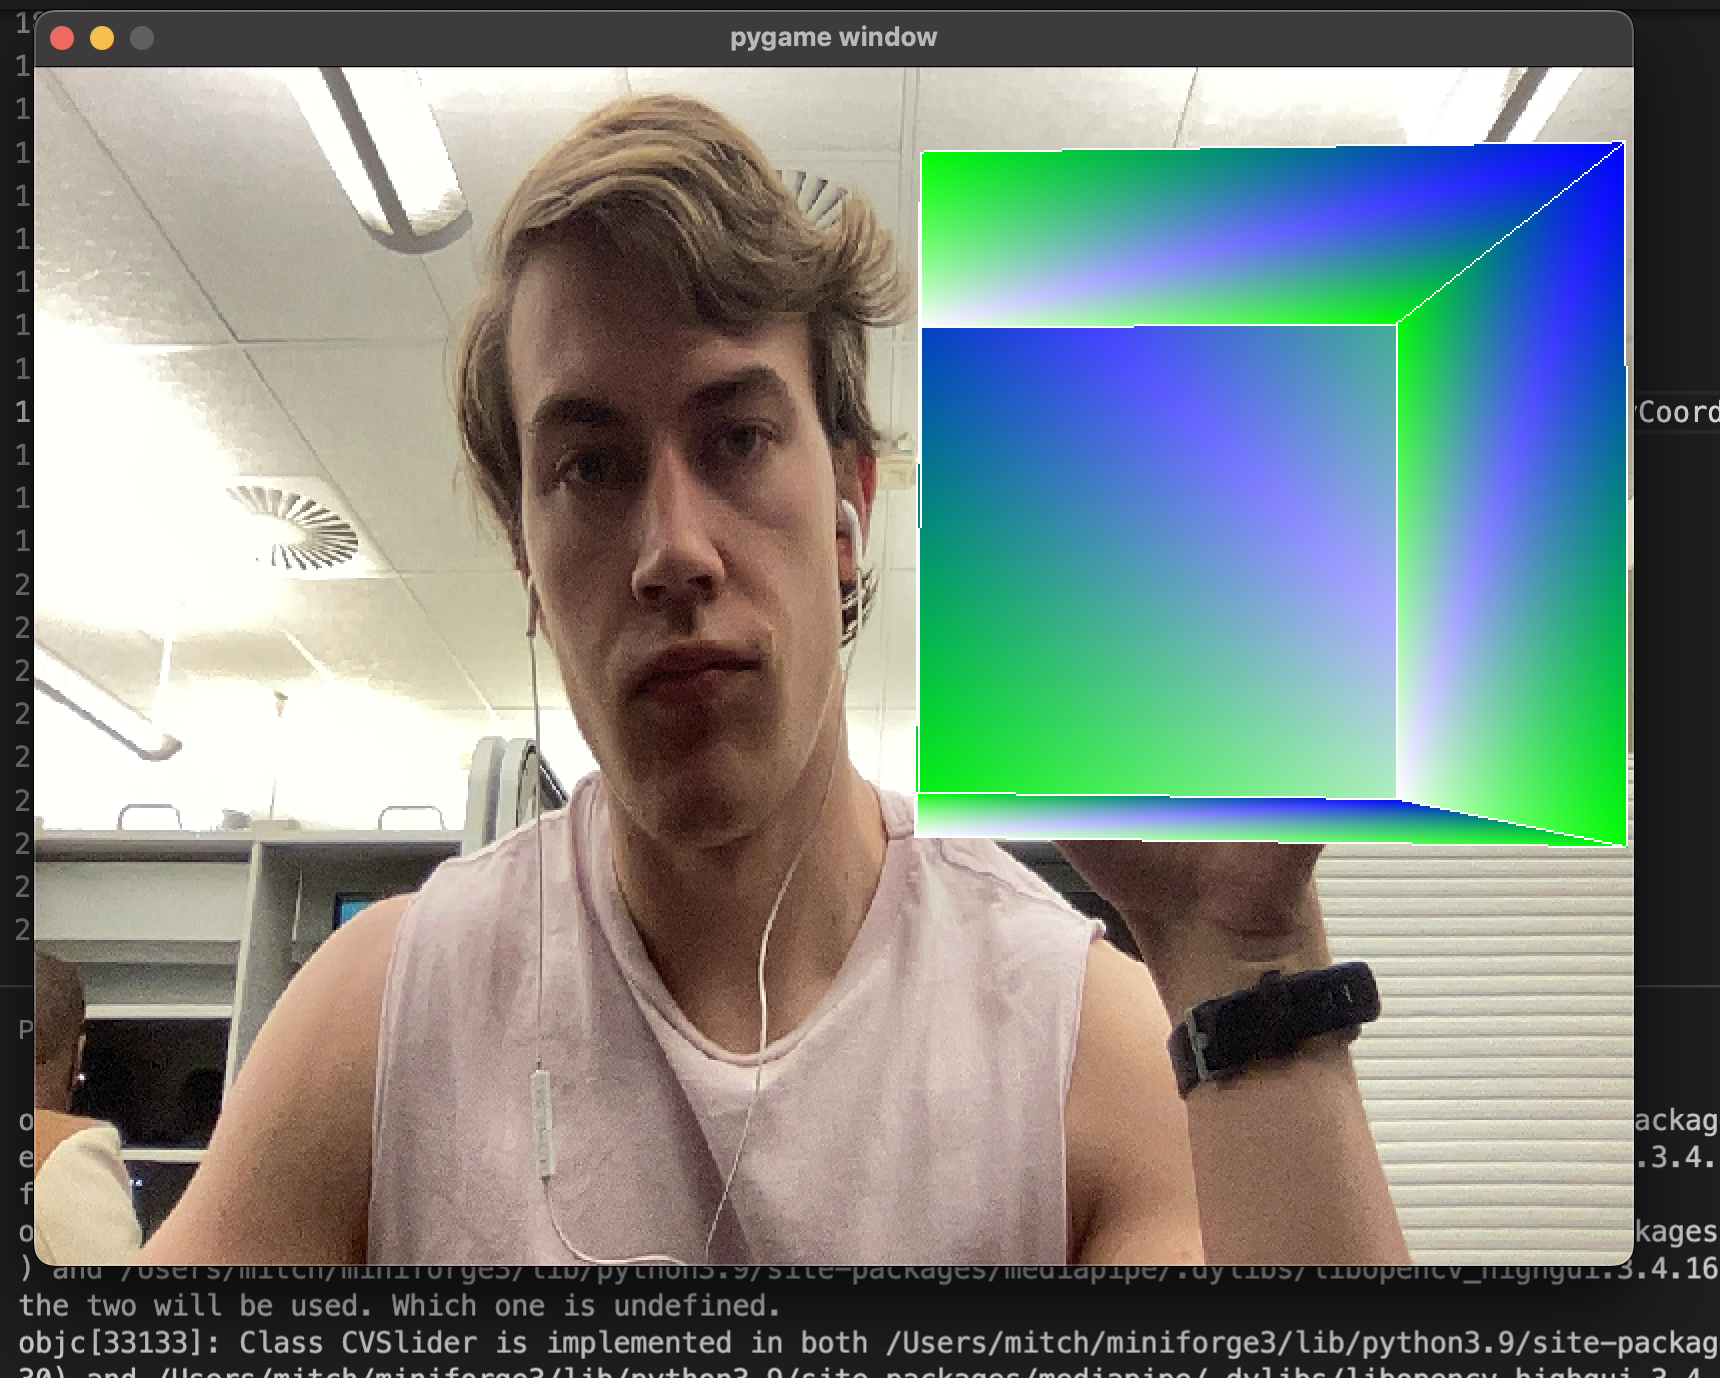
\includegraphics[width=0.6\linewidth]{figures/OpenGL Mediapipe Cube.png}
    \caption{Output of the OpenGL and Mediapipe hands prototype application}
    \label{fig:OpenGL Mediapipe Cube}
\end{figure}

\section[2022/06/07]{Tuesday, 07 June 2022}

\subsection{OpenGL And Mediapipe Prototyping}

In order to arrive at the end of the semester with a working prototype assembled from prebuilt components, the integration of Mediapipe Hands and the OpenGL cube rendering program was undertaken and its implementation detailed here. \\

Mediapipe hands has been used in earlier prototypes for hand detection and will again be used now to generate a three dimensional model of the user's hand from webcam input. Earlier prototypes utilized the Javascript version of mediapipe hands since the Apple Silicon API could not be installed but after much trial and error this was rectified and simplified the process a lot - a single Python file could now be written that combines the OpenGL cube rendering prototype with the mediapipe hand detection model that tracks the co-ordinates of a user's fingers and utilizes it as input for the cube's position on the screen. The output of the mediapipe Python example file can be seen in \FigRef{fig:python_mediapipe_hands}.\\

\begin{figure}[h]
    \centering
    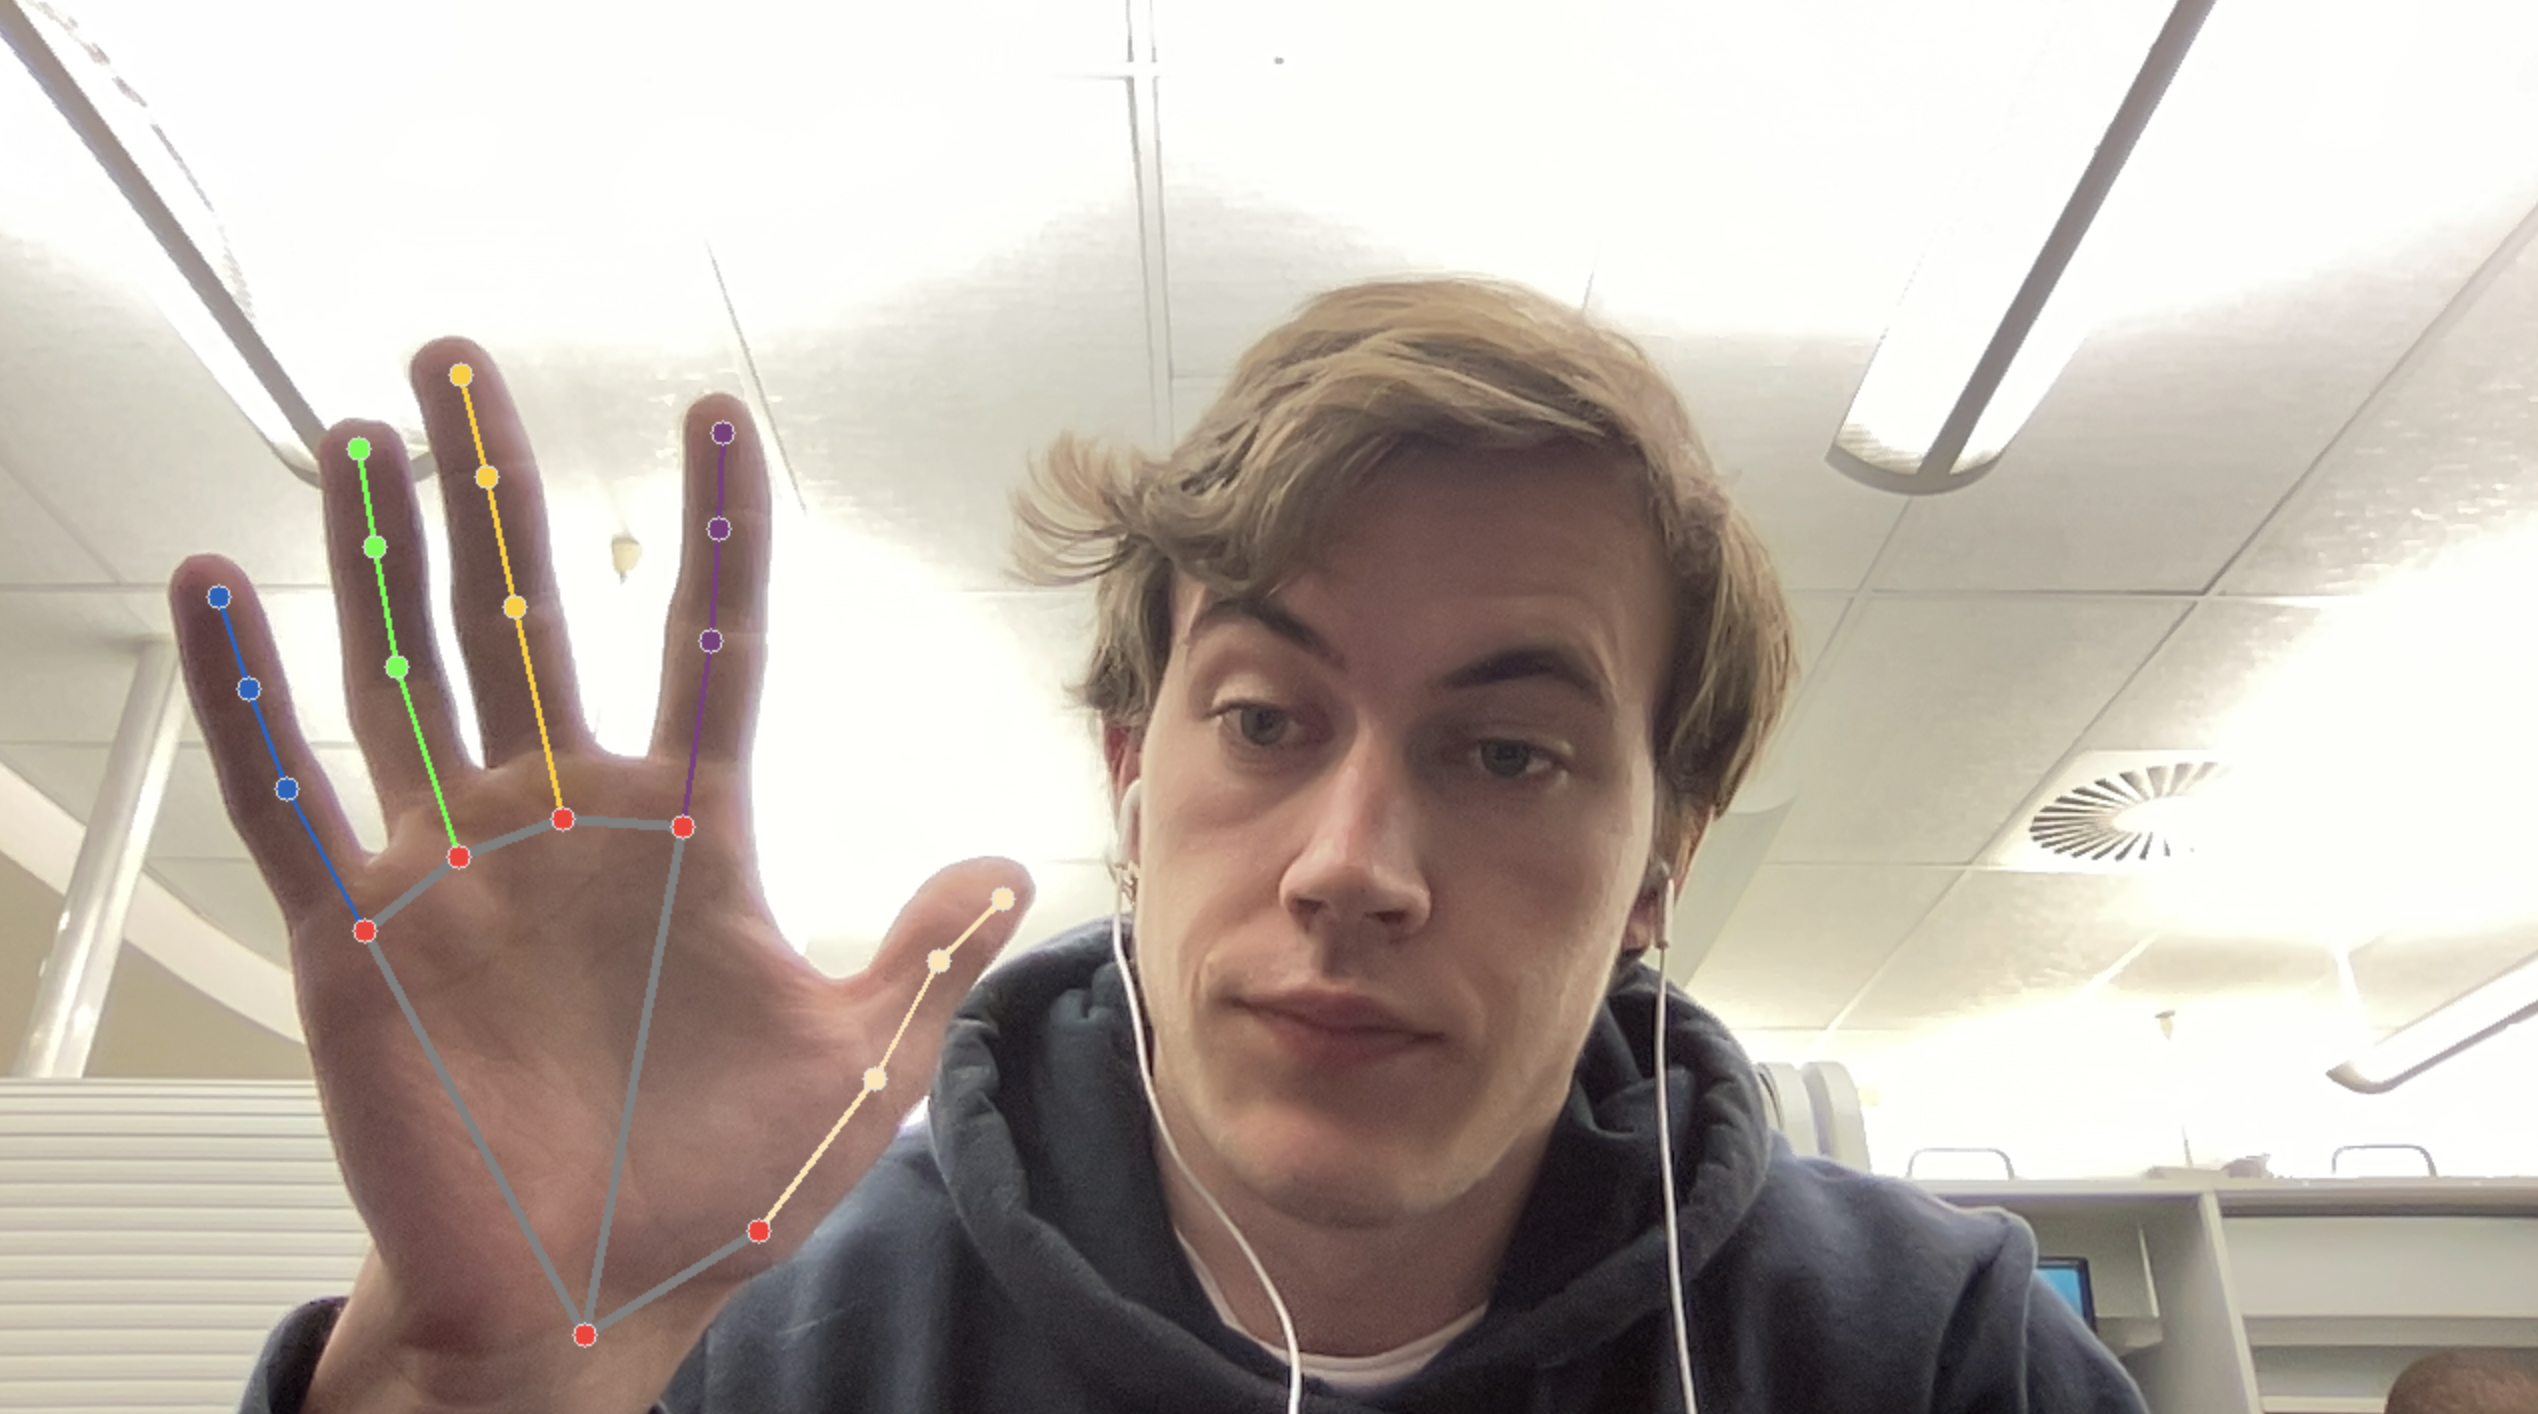
\includegraphics[width=0.6\linewidth]{figures/python_mediapipe_hands.png}
    \caption{Output of the Mediapipe hands python example application}
    \label{fig:python_mediapipe_hands}
\end{figure}

A video demonstration of the prototype's functioning can be found in the Project's repository under Prototypes but the system was able to accurately take the location of the user's pinky using mediapipe and the code

\begin{lstlisting}
    pinkyCoords = hand_landmarks.landmark[20]
  \end{lstlisting}

and use that as input to the OpenGl translate and rotation commands which scaled and adjusted the cube in order to try and be placed on top of the user's hand. This was accomplished with 

\begin{lstlisting}
    glTranslatef(-(lastX-pinkyCoords.x)*1.5, -(lastY-pinkyCoords.y)*1.5, -(lastZ-pinkyCoords.z)*1.5)
    glRotatef(1, -(lastX-pinkyCoords.x)*1.5, -(lastY-pinkyCoords.y)*1.5, 0.0)
  \end{lstlisting}

PyGame was utilized to display the OpenGL rendering as well as mediapipe hands regression output. Further refinement is needed to move the cube at the speed the user moves their hand and to be closer to the user's hand rather than further away. Depth information from the Kinect sensor also needs to be considered in order to create a synthetic representation of the environment that can be compared against and used to perform collision avoidance and realistic physics additions to the prototype such as the mimicking of gravity or outside influences on the cube.

\section[2022/06/17]{Friday, 17 June 2022}

\subsection{Project Proposal Revision}

The aim of this work session is to revise the project proposal according to Prof. Hanekom's feedback on the first submission and to clarify certain aims of the project with regards to the processing platform it will be conducted on.\\


The main area of concern regarding the first proposal submission was the processing platform. As per an email dated Friday 17th June with Mr. Grobler (see Appendix) it was determined that an embedded platform should be used in the project and that "certain aspects be demonstrated on the platform." However, it is expected that in order to achieve the necessary requirements and specifications outlined in the proposal that a PC platform will have to be used. Following from this, it was decided to update the proposal with the use of the embedded platform as the main processing platform but specify in the implementation section that the main challenge of the project will be to achieve the system's functioning on an embedded platform due to the computationally intensive nature of the gesture control algorithm and virtual object rendering.\\

It is expected that an embedded platform that falls within the three-thousand rand budget of the project will be unsuitable to achieve the performance described in the specifications as they were initially developed in the first proposal submission assuming a PC platform would be used for processing. It is hypothesized however that just the gesture recognition algorithm could be optimized to the point where it could run effectively and meet specifications on a standard embedded platform like a Pandaboard or Odroid. The gesture recognition system may also be able to run slowly on the same platform with a much reduced frame rate. The use of two embedded platforms in tandem - one running the gesture recognition system and the other the virtual object rendering could be a possible way to achieve the performance specifications on an embedded platform but it is doubtful if this could be accomplished within the budget. 

The following additional points of feedback were given about the proposal. The incorrect fonts were used in the proposal and this has been rectified by adhering more strictly to the proposal template. Requirement 6 of the system requirements and specifications was marked as a redundant specification. This specification stated that 9 known gesture templates had to stored in memory - this was implied earlier by requirement 2 where the system was expected to be able to recognize 9 discrete gestures. The requirement has thus been removed. Requirement 1 stated that user's hand gestures and corresponding changes to the position and orientation of the virtual object would have a latency of less than 41.6ms. However, it was not explained why this was the case - standard filmmaking techniques utilize standard frame rates that update the picture displayed on a screen 24 or 30 frames per second.\\

Values less than 24fps make video footage appear choppy or disjointed to the human eye because below this value the brain struggles to simulate \href{https://gamut.io/why-frame-rate-matters-24fps-vs-30fps/}{"fluid motion."} Thus it is necessary to use at least 24fps for the virtual object rendering system and gesture recognition system otherwise the illusion of real-time virtual object control will be destroyed. Higher frame rates than 24fps will appear to make the virtual object move more smoothly but would require a corresponding increase in the amount of inferrences for the hand gesture detection system and since the embedded system is already expected to have difficulties meeting the 24fps specifications it was decided that this should remain the target refresh rate of both the virtual object rendering algorithm and gesture detection algorithm. The motivation in requirement 1 was updated to reflect this reasoning. \\

In the description of what the off-the-shelf components of the system would be, there was concern in requirement 1 about what constituted "video processing libraries" as only "basic low-level operations may be done with the assistance of libraries." The requirement was updated to reflect that the only libraries to be used off-the-shelf will be those used for video capture, image to array conversion and image display to the user. Finally, in the Design and Implementation Tasks section of the proposal, the use of the imperative form to describe individual design and implementation tasks was criticized - the grammar of this section has thus been rectified to remove use of the imperative form.\\

In conclusion, the system is expected to function on an embedded platform but with severe performance deficiencies due to the computationally straining nature of rendering 3D video alongside a system that can accept two streams of video input and perform gesture recogniton on one of those streams of input. Conducting only the gesture recognition computations on the embedded platform is expected to be doable and the potential use of multiple embedded platforms is a potential way of fulfilling the project specifications in their new form.\\